\subsection{Import ASTERIX from Network}
\label{sec:ui_import_asterix_network}

This task allows importing ASTERIX data from the network into the opened database, and switches from 'Offline' to 'Live' mode. \\

\begin{figure}[H]
    \centering
    \hspace*{-1.5cm}
    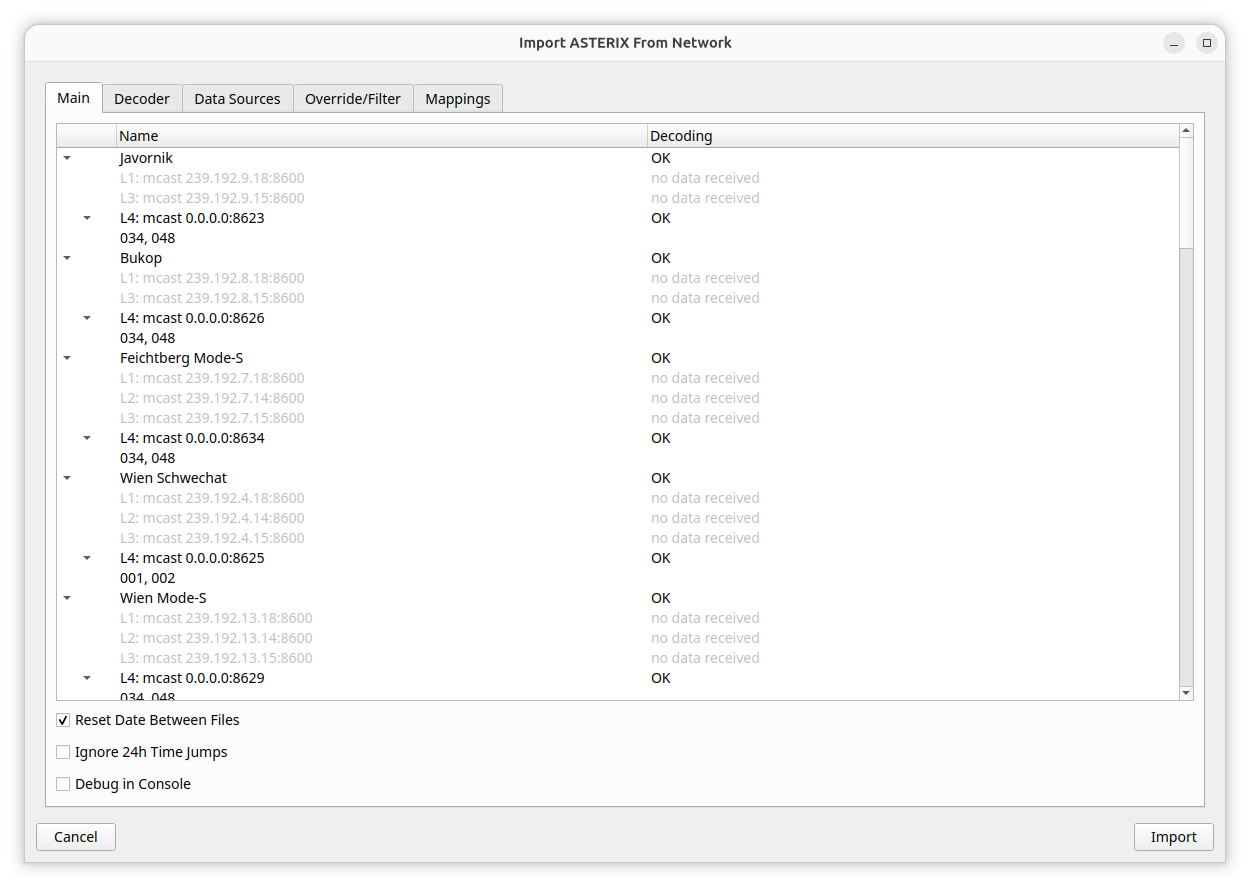
\includegraphics[width=18cm]{figures/asterix_import_data_network.png}
  \caption{Import ASTERIX Data from network}
\end{figure}

Except for the differing ASTERIX source at the top, everything works the same as described in \nameref{sec:ui_import_asterix}. \\

The following items exist:
\begin{itemize}
\item Reset Date Between Files: Not used
\item Ignore 24h Time Jumps: Do not detect 24h time jumps in input data - import everything into same date
\item Debug in Console: Additional debugging information is output to the console, and the ASTERIX decoding is switched to single-threading for easier investigation
\end{itemize}
\ \\

\paragraph{How Network Lines Are Used}

The task collects the \texttt{network\_lines} entries from every data source in the active Data Context and opens one UDP Receiver per (data source, line). Lines are configured per data source under \nameref{sec:configure_datasources_network}. \\

Each data source supports up to four network lines, keyed \texttt{L1} to \texttt{L4}. A line carries the following parameters:

\begin{itemize}
  \item \texttt{mcast\_ip}: Required. The bind address of the UDP socket. Either a multicast group (224.0.0.0 to 239.255.255.255) or a unicast / any address (\texttt{0.0.0.0} or a local host IP) for direct UDP reception.
  \item \texttt{mcast\_port}: Required. The UDP port to bind.
  \item \texttt{listen\_ip}: Optional. The local interface IP used to bind and to join the multicast group on. Recommended whenever \texttt{mcast\_ip} is a real multicast group; without it, the OS picks the interface and the wrong NIC may be chosen.
  \item \texttt{sender\_ip}: Optional. If set, only datagrams whose source address equals this value are forwarded to the importer; all others are silently dropped.
\end{itemize}
\ \\

For each line, the receiver:
\begin{itemize}
  \item Opens a UDP socket with \texttt{SO\_REUSEADDR} (so multiple data sources can share a port).
  \item Binds to \texttt{mcast\_ip:mcast\_port}.
  \item If \texttt{mcast\_ip} is a multicast group, joins the group (on the \texttt{listen\_ip} interface if set).
  \item If \texttt{sender\_ip} is set, filters incoming datagrams by source address.
\end{itemize}
\ \\

\paragraph{Example Line Configurations}

\textbf{1. Multicast with explicit interface (typical operational setup).} Bind to a multicast group, join on a specific NIC.

\begin{lstlisting}
"L1": {
  "mcast_ip":  "239.192.9.18",
  "mcast_port": 8600,
  "listen_ip": "192.168.10.5"
}
\end{lstlisting}

\textbf{2. Multicast without explicit interface.} Same as above, but the OS picks the interface used to join the group.

\begin{lstlisting}
"L1": {
  "mcast_ip":  "239.192.9.18",
  "mcast_port": 8600
}
\end{lstlisting}

\textbf{3. Local replay on any interface.} \texttt{0.0.0.0} binds on all interfaces, accepting any UDP traffic that arrives on the port. Useful for local playback tools sending to \texttt{127.0.0.1} or to the host's own IP.

\begin{lstlisting}
"L4": {
  "mcast_ip":  "0.0.0.0",
  "mcast_port": 8623
}
\end{lstlisting}

\textbf{4. Local replay bound to a specific host IP.} Binds only on the given NIC; useful when the playback source addresses one specific interface of the COMPASS host.

\begin{lstlisting}
"L1": {
  "mcast_ip":  "192.168.0.171",
  "mcast_port": 5001,
  "listen_ip": "192.168.0.171"
}
\end{lstlisting}

\textbf{5. Multicast with sender filter.} Any of the above can be combined with \texttt{sender\_ip} to accept only datagrams from one source, e.g. when several systems share a multicast group.

\begin{lstlisting}
"L1": {
  "mcast_ip":  "239.192.9.18",
  "mcast_port": 8600,
  "listen_ip": "192.168.10.5",
  "sender_ip": "192.168.10.20"
}
\end{lstlisting}


\includegraphics[width=0.5cm]{../../data/icons/hint.png} \textbf{Please note that} for real multicast addresses (224.0.0.0 to 239.255.255.255) it is strongly recommended to also set \texttt{listen\_ip} to the local address of the network interface to be used. Otherwise the multicast data might not be received, or the wrong network interface might be picked up, causing COMPASS to receive no data. \\

When the import is started, data is continuously read from the network (according to the data source network lines specification) and processed according to \nameref{sec:live_mode}.
